\documentclass[english, 11pt]{article}
\usepackage{graphicx}
\usepackage{amsmath}
\usepackage{hyperref}
\usepackage{setspace}
\usepackage{apacite}
\usepackage{hyperref}
\usepackage[sort]{natbib}
\usepackage{pxfonts}
\usepackage[utf8]{inputenc}
\usepackage[left=1in,right=1in,top=1in,bottom=1in]{geometry}
\usepackage[left]{lineno}
\usepackage{soul}
\linenumbers

\newcommand{\synthThirds}{S1}
\newcommand{\accuracyNetworks}{S2}
\newcommand{\componentsNetworks}{S3}

\title{High-order cognition is supported by information-rich but compressible brain activity patterns}

\author{Lucy L. W. Owen\textsuperscript{1, 2} and Jeremy R. Manning\textsuperscript{1,
*}\\\textsuperscript{1}Department of Psychological and Brain Sciences,\\Dartmouth College,
Hanover, NH\\[0.1cm]\textsuperscript{2}Carney Institute for Brain Sciences,\\Brown University,
Providence, RI\\[0.1cm] \textsuperscript{*}Address correspondence to
jeremy.r.manning@dartmouth.edu}

\begin{document}
\maketitle


\begin{abstract} 

We applied dimensionality reduction algorithms and pattern classifiers to
functional neuroimaging data collected as participants listened to a story,
temporally scrambled versions of the story, or underwent a resting state
scanning session. These experimental conditions were intended to require
different depths of processing and inspire different levels of cognitive
engagement. We considered two primary aspects of the data. First, we treated
the maximum achievable decoding accuracy across participants as an indicator of
the ``informativeness'' of the recorded patterns. Second, we treated the number
of features (components) required to achieve a threshold decoding accuracy as a
proxy for the ``compressibility'' of the neural patterns (where fewer
components indicate greater compression). Overall, we found that the peak
decoding accuracy (achievable without restricting the numbers of features)
was highest in the intact (unscrambled) story listening condition.  However, the
number of features required to achieve comparable classification accuracy
was also lowest in the intact story listening condition.  Taken together, our work
suggests that our brain networks flexibly reconfigure according to ongoing task
demands, and that the activity patterns associated with higher-order cognition
and high engagement are both more informative and more compressible than the
activity patterns associated with lower-order tasks and lower levels of
engagement.

\bigskip
\noindent
\textbf{Keywords: information, compression, temporal decoding, dimensionality
reduction, neuroimaging}

\end{abstract}

\doublespacing

\section*{Introduction}

Large-scale networks, including the human brain, may be conceptualized as
occupying one or more positions along on a continuum. At one extreme, every
node is fully independent from every other node. At the other extreme, all
nodes behave identically. Each extreme optimizes key properties of how the
network functions. When every node is independent, the network is maximally
\textit{expressive}: if we define the network's ``state'' as the activity
pattern across its nodes, then every state is equally reachable by a network
with fully independent nodes. On the other hand, a network of identically
behaved nodes optimizes \textit{robustness}: any subset of nodes may be removed
from the network without any loss of function or expressive power, as long as
any single node remains. Presumably, most natural systems tend to occupy
positions between these extremes. We wondered: might the human brain
reconfigure itself to be more flexible or more robust according to ongoing
demands? In other words, might the brain reconfigure its connections or
behaviors under different circumstances to change its position along this
continuum?

Closely related to the above notions of expressiveness versus robustness are
measures of how much \textit{information} is contained in a given signal or
pattern, and how \textit{redundant} a signal is~\citep{Shan48}. Formally,
information is defined as the amount of uncertainty about a given variables'
outcomes (i.e., entropy), measured in \textit{bits}, or the optimal number of
yes/no questions needed to reduce uncertainty about the variable's outcomes to
zero. Highly complex systems with many degrees of freedom (i.e., high
flexibility and expressiveness), are more information-rich than simpler or more
constrained systems. The redundancy of a signal denotes the difference between
how expressive the signal \textit{could} be (i.e., proportional to the number
of unique states or symbols used to transmit the signal) and the actual
information rate (i.e., the entropy of each individual state or symbol). If a
brain network's nodes are fully independent, then the number of bits required
to express a single activity pattern is proportional to the number of nodes.
The network would also be minimally redundant, since the status of every node
would be needed to fully express a single brain activity pattern. If a brain
network's nodes are fully coupled and identical, then the number of bits
required to express a single activity pattern is proportional to the number of
unique states or values any individual node can take on. Such a network would
be highly redundant, since knowing any individual node's state would be
sufficient to recover the full-brain activity pattern. Highly redundant systems
are also robust, since there is little total information loss due to removing
any given observation.

We take as a given that brain activity is highly flexible: our brains can
exhibit nearly infinite activity patterns. This flexibility implies that our
brains activity patterns are highly information rich. However, brain activity
patterns are also highly structured. For example, full-brain correlation
matrices are stable within~\citep{FinnEtal15, FinnEtal17, GratEtal18} and
across~\citep{YeoEtal11, GlerEtal12, GratEtal18, ColeEtal14} individuals. This
stability suggests that our brains' activity patterns are at least partially
constrained, for example by anatomical, external, or internal factors.
Constraints on brain activity that limit its flexibility decrease
expressiveness (i.e., its information rate). However, constraints on brain
activity also increase its robustness to noise (e.g., ``missing'' or corrupted
signals may be partially recovered). For example, recent work has shown that
full-brain activity patterns may be reliably recovered from only a relatively
small number of implanted electrodes~\citep{OwenEtal20, ScanEtal21}. This
robustness property suggests that the relevant signal (e.g., underlying factors
that have some influence over brain activity patterns) are compressible.

\begin{figure}[tp]

  \centering
  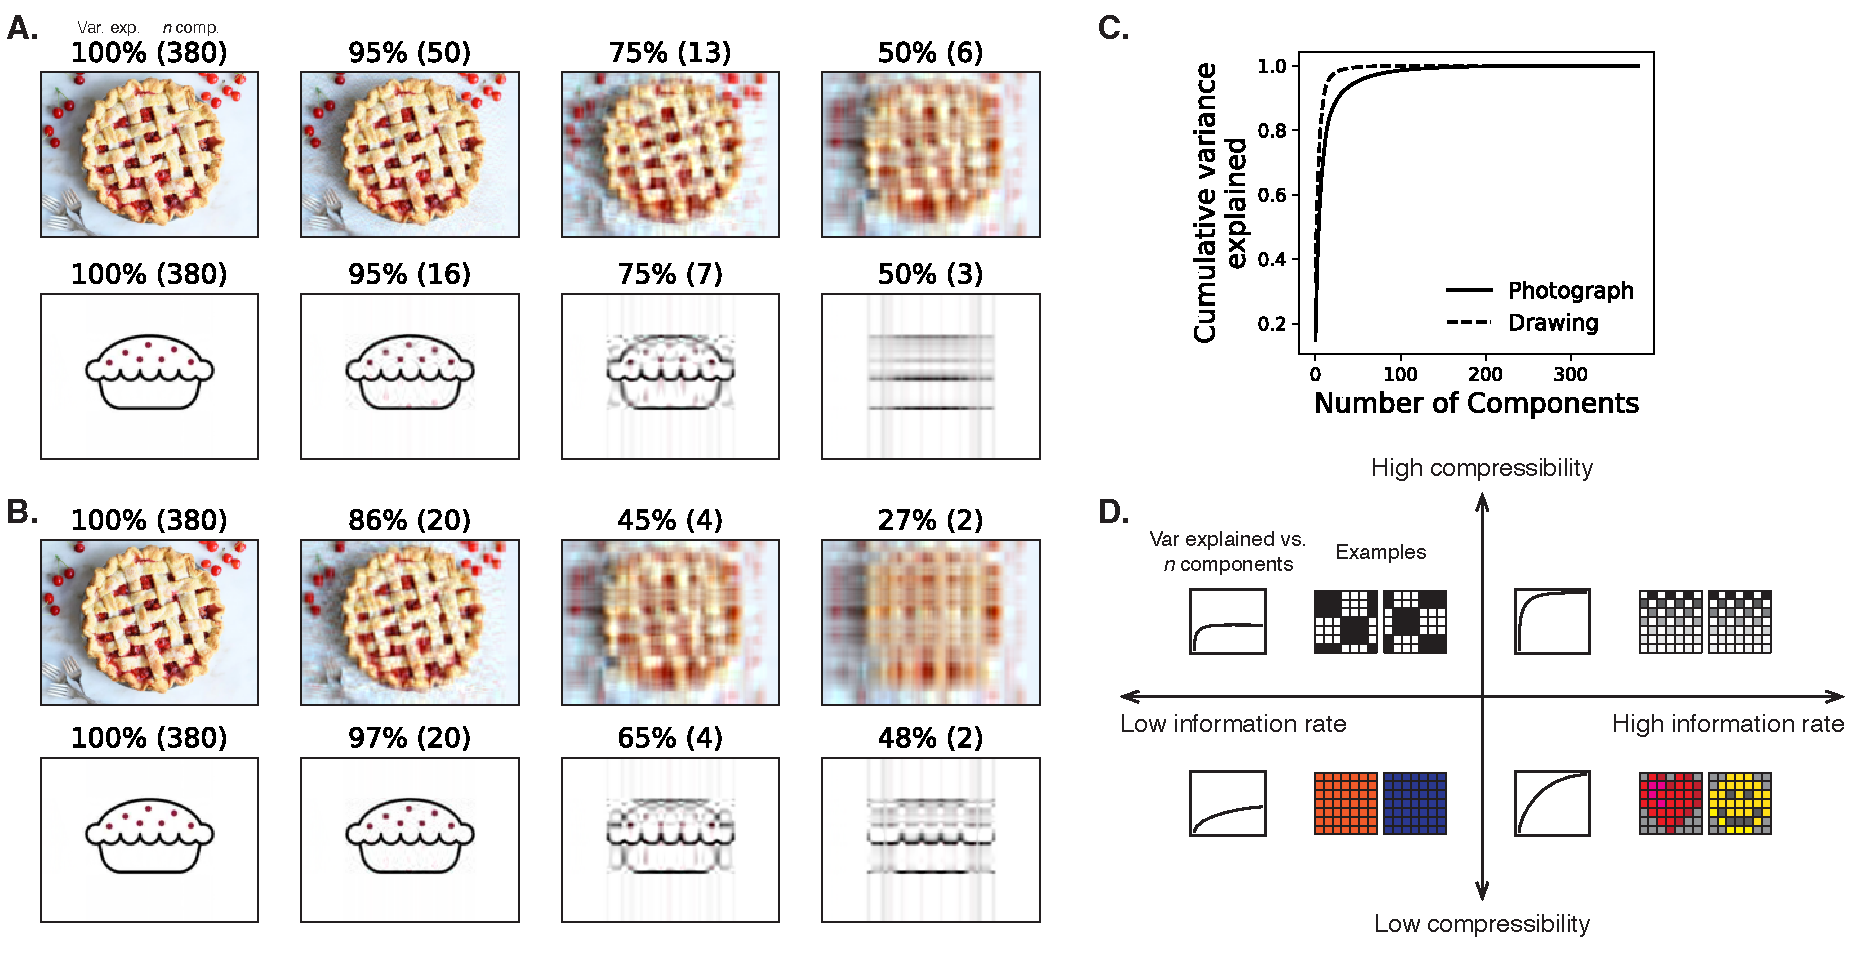
\includegraphics[width=\textwidth]{figs/information_and_compressibility}
  
  \caption{\textbf{Information content and compressibility.} \textbf{A.
  Variance explained for two images.} We applied principal components analysis
  to a photograph and drawing, treating the rows of the images as
  ``observations.'' Across columns, we identified the numbers of components
  required to explain 100\%, 95\%, 75\%, or 50\% of the cumulative variance in
  each image (the 100\% columns denote the original images). The numbers of
  components are indicate in parentheses, and the resulting ``compressed''
  images are displayed. \textbf{B. Representing two images with different
  numbers of components.} Using the same principal component decompositions as
  in Panel A, we computed the cumulative proportion of variance explained with
  380 (original images), 20, 4, or 2 components. \textbf{C. Cumulative variance
  explained versus number of components.} For the images displayed in Panels A
  and B, we plot the cumulative proportion of variance explained as a function
  of the number of components used to represent each image. \textbf{D.
  Information rate and compressibility.} Across multiple images, the
  information rate (i.e., the amount of information contained in each image;
  horizontal axis) is high when each individual pixel provides information that
  cannot be inferred from other pixels. High-information rate images tend to be
  high-resolution, and low-information rate images tend to be low-resolution.
  Compressibility is related to the difference between the information required
  to specify the original versus compressed images (vertical axis). Highly
  compressible images often contain predictable structure (redundancies) that
  can be leveraged to represent the images much more efficiently than in their
  original feature spaces.}

\label{fig:information-compression} 
\end{figure}

To the extent that brain activity patterns contain rich task-relevant
information, we should be able to use the activity patterns to accurately
differentiate between different aspects of the task~\citep[e.g., using pattern
classifiers;][]{NormEtal06b}. For example, prior work has shown a direct
correspondence between classification accuracy and the information content of a
signal~\citep{Alva02}. To the extent that brain activity patterns are
compressible, we should be able to generate simplified (e.g., lower
dimensional) representations of the data while still preserving the relevant or
important aspects of the original signal. In general, information content and
compressibility are related but are partially dissociable
(Fig.~\ref{fig:information-compression}). If a given signal (e.g., a
representation of brain activity patterns) contains more information about
ongoing cognitive processes, then the peak decoding accuracy should be high.
And if the signal is compressible, a low-dimensional embedding of the signal
will be similarly informative to the original signal
(Fig.~\ref{fig:information-compression}D).


Several recent studies suggest that the complexity of brain activity is
task-dependent, whereby simpler tasks with lower cognitive demands are
reflected by simpler and more compressible brain activity patterns, and more
complex tasks with higher cognitive demands are reflected by more complex and
less compressible brain activity patterns~\citep{MackEtal20, OwenEtal21}. These
findings complement other work suggesting that functional connectivity
(correlation) patterns are task-dependent~\citep{FinnEtal17, OwenEtal20,
ColeEtal14}, although see~\cite{GratEtal18}. Higher-order cognitive processing
of a common stimulus also appears to drive more stereotyped task-related
activity and functional connectivity across individuals~\citep{HassEtal08,
LernEtal11, SimoChan20, SimoEtal16}.

The above studies are consistent with two potential descriptions of how
cognitive processes are reflected in brain activity patterns. One possibility
is that the information rate of brain activity increases during more complex or
higher-level cognitive processing. If so, then the ability to reliably decode
cognitive states from brain activity patterns should improve with task
complexity or with the level (or ``depth'') of cognitive processing. A second
possibility is that the compressibility of brain activity patterns increases
during more complex or higher-level cognitive processing. If so, then
individual features of brain recordings, or compressed representations of brain
recordings, should carry more information during complex or high-level (versus
simple or low-level) cognitive tasks.

We used a previously collected neuroimaging dataset to estimate the extent to
which each of these two possibilities might hold. The dataset we examined
comprised functional magnetic resonance imaging (fMRI) data collected as
participants listened to an audio recording of a 10-minute story, temporally
scrambled recordings of the story, or underwent a resting state
scan~\citep{SimoEtal16}. Each of these experimental conditions evokes different
depths of cognitive processing~\citep{SimoEtal16,LernEtal11,
HassEtal08,OwenEtal21}. We used across-participant classifiers to decode
listening times in each condition, as a proxy for how ``informative'' the
task-specific activity patterns were~\citep{SimoChan20}. We also use principle
components analysis to generate lower-dimensional representations of the
activity patterns. We then repeated the classification analyses after
preserving different numbers of components and examined how classification
accuracy changed across the different experimental conditions.



\section*{Results}

We sought to understand whether higher-level cognition is reflected by more
reliable and informative brain activity patterns, and how compressibility of
brain activity patterns relates to cognitive complexity. We developed a
computational framework for systematically assessing the informativeness and
compressibility of brain activity patterns recorded under different cognitive
circumstances. We used across-participant decoding accuracy (see
\textit{Forward inference and decoding accuracy}) as a proxy for
informativeness. To estimate the compressibility of the brain patterns, we used
group principal components analysis (PCA) to project the brain patterns into
$k$-dimensional spaces, for different values of $k$ (see \textit{Hierarchical
Topographic Factor Analysis (HTFA)} and \textit{Principal components analysis
(PCA)}). For more compressible brain patterns, decoding accuracy should be more
robust to small values of $k$.

We analyzed a dataset collected by \cite{SimoEtal16} that comprised four
experimental conditions. These conditions exposed participants to stimuli that
systematically varied in cognitive engagement. In the \textit{intact}
experimental condition, participants listened to an audio recording of a
10-minute story. In the \textit{paragraph}-scrambled experimental condition,
partipants listened to a temporally scrambled version of the story, where the
paragraphs occurred out of order, but where the same set of paragraphs was
presented over the entire listening interval. All participants in this
condition experienced the scrambled paragraphs in the same order. In the
\textit{word}-scrambled experimental condition, participants listened to a
temporally scrambled version of the story, where the words occurred in a random
order. Again, all participants in this condition experienced the scrambled
words in the same order. Finally, in the \textit{rest} experimental condition,
participants lay in the scanner with no overt stimulus, while keeping their
eyes open and blinking as needed. This public dataset provided a convenient
means for testing our hypothesis that different levels of cognitive processing
and engagement affect how informative and compressible the associated brain
patterns are.

\begin{figure}[tp]
  \centering
  
  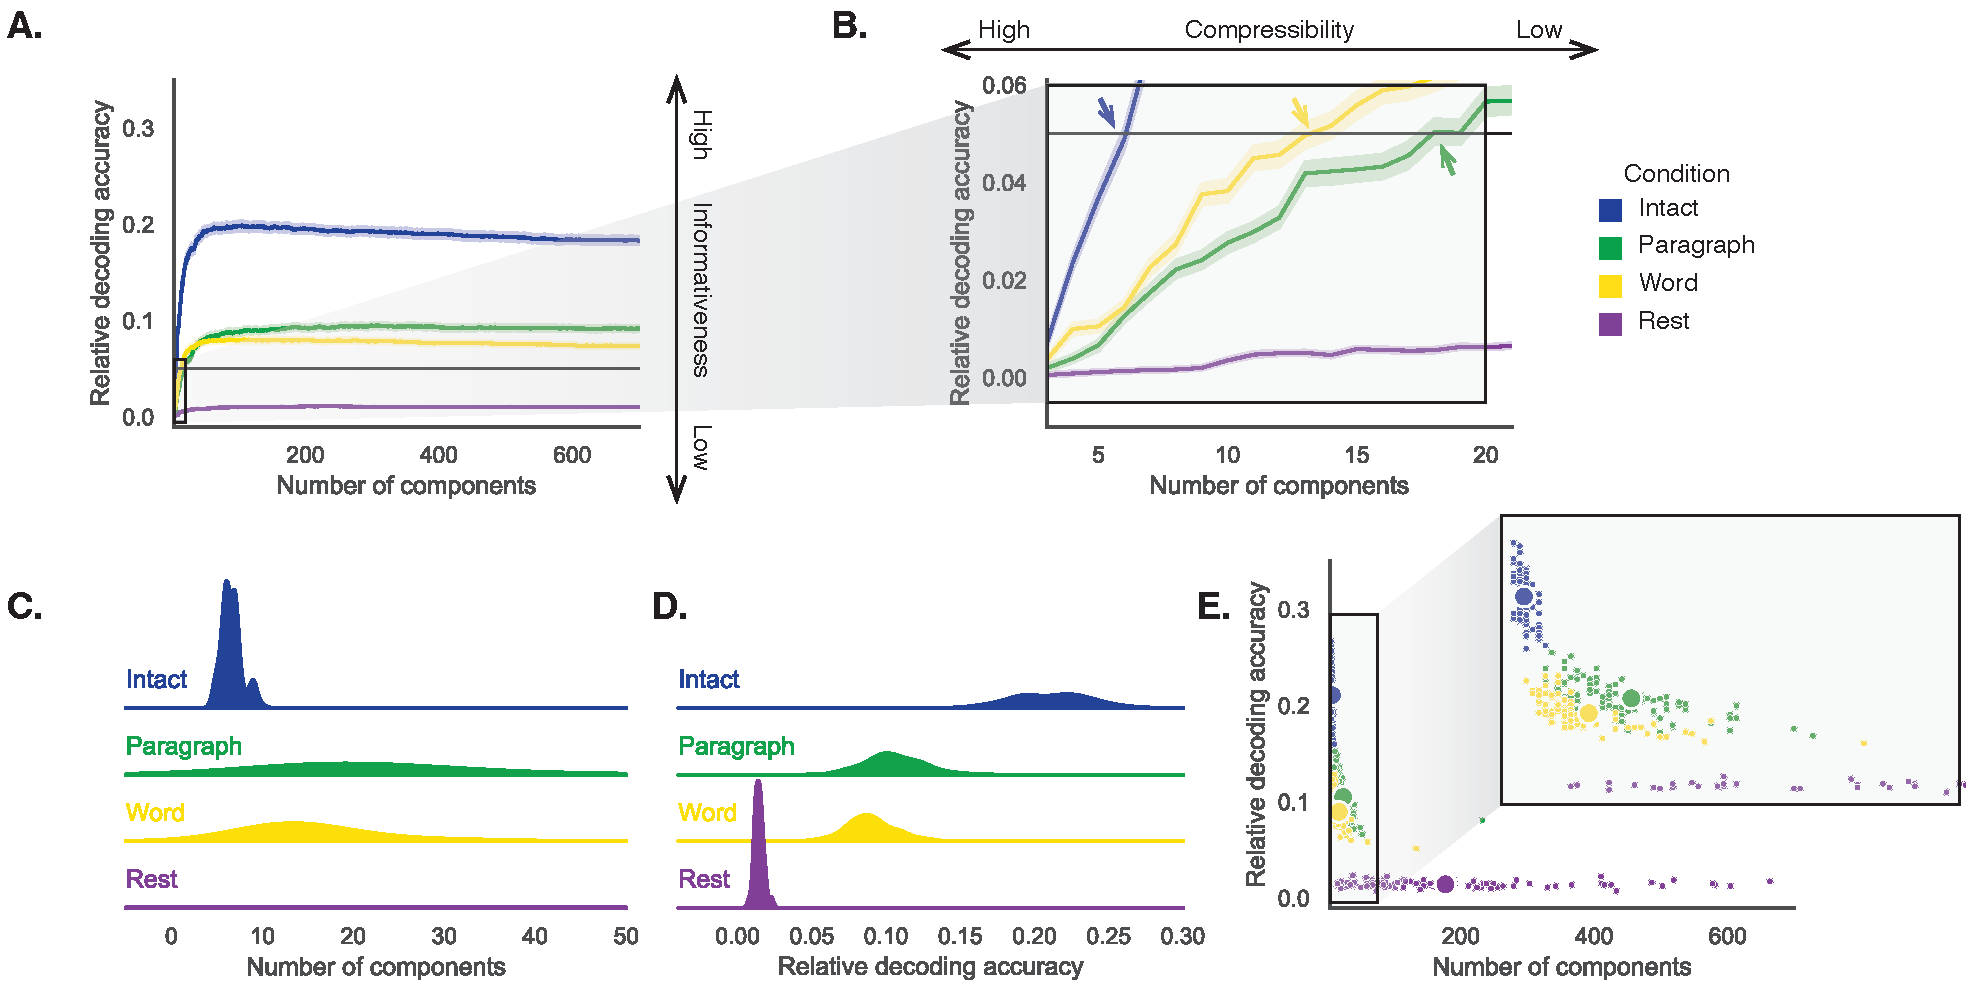
\includegraphics[width=0.8\textwidth]{figs/decoding_and_inflection}

\caption{\textbf{Decoding accuracy and compression.} \textbf{A. Decoding
accuracy by number of components.} Ribbons of each color display
cross-validated decoding performance for each condition (intact, paragraph,
word, and rest), as a function of the number of components (features) used to
represent the data. The horizontal red line denotes chance performance, and the
horizontal black line denotes 5\% decoding accuracy (used as a reference in
Panel B). \textbf{B. Numbers of components required to reach a fixed decoding
accuracy threshold, by condition.} The panel displays a zoomed-in view of the
inset in Panel A. Intersections between each condition's decoding accuracy
curve and the 5\% decoding accuracy reference line are marked by arrows.
\textbf{C. Estimating inflection points.} We sought to identify an ``inflection
point'' for each decoding curve, denoting the number of components at which the
decoding curve asymptotes. We fit sigmoid functions to each decoding curve
(left sub-panel) and then computed the minimum number of components for which
the second derivative of the sigmoid was both positive and less than a
threshold value of 0.0001. \textbf{D. Inflection points by condition.} Each dot
displays the number of components ($x$-axis) and decoding accuracy ($y$-axis)
at one condition's inflection point. All error ribbons denote
bootstrap-estimated 95\% confidence intervals.}

\label{fig:inflection}
\end{figure}

To evaluate the relation between informativeness and compressibiilty for brain
activity from each experimental condition, we trained a series of
across-participant temporal decoders on compressed representations of the data.
Figure~\ref{fig:inflection}A displays the decoding accuracy as a function of
the number of principal components used to represent the data. Several patterns
were revealed by the analysis. First, in general (i.e., across experimental
conditions), decoding accuracy improves as the number of components increases.
However, decoding accuracy peaked at higher levels for experimental conditions
that exposed participants to cognitively richer stimuli. The peak decoding
accuracy was highest for the ``intact'' condition (versus paragraph: $t(XXX) =
XXX, p = XXX$; versus word: $t(XXX) = XXX, p = XXX$; versus rest: $t(XXX) =
XXX, p = XXX$), next highest for the ``paragraph'' condition (versus word:
$t(XXX) = XXX, p = XXX$; versus rest: $t(XXX) = XXX, p = XXX$), and next
highest for the ``word'' condition (versus rest: $t(XXX) = XXX, p = XXX$). This
ordering implies that cognitively richer conditions evoke more stable brain
activity patterns across people.

The cognitively richer conditions also displayed steeper initial slopes. For
example, the intact condition decoders reached an arbitrarily chosen threshold
of 5\% accuracy using fewer components than the paragraph condition decoders
($t(XXX) = XXX, p = XXX$) or word condition decoders ($t(XXX) = XXX, p = XXX$),
and decoding accuracy never exceeded 5\% for the rest condition. This suggests
that brain activity patterns evoked by cognitively richer conditions are more
compressible, such that representing the data using the same number of
principal components provides more information to the temporal decoders
(Fig.~\ref{fig:inflection}B).

In every experimental condition, decoding accuracy appeared to asymptote (i.e.,
hit an upper limit) beyond some characteristic number of components that
differed across conditions. To quantify the ``inflection points'' at which the
decoding curves in Figure~\ref{fig:inflection}A flattened out, we fit a sigmoid
function to the average decoding curve for each condition. We defined the
inflection point for each condition as the point on the fitted sigmoid where
the second derivative was both positive and less than a threshold value of
0.0001 (i.e., approaching 0 from the right). These inflection points reflect a
``balance'' between higher decoding accuracy (which tends to be better when
more components are used) and compression (which is better for fewer
components). Plotting each condition's inflection point
(Fig.~\ref{fig:inflection}D) reveals that both the number of components and the
decoding accuracy at each inflection point increase systematically across
conditions in proportion to cognitive richness.


\begin{figure}[tp]
  \centering
  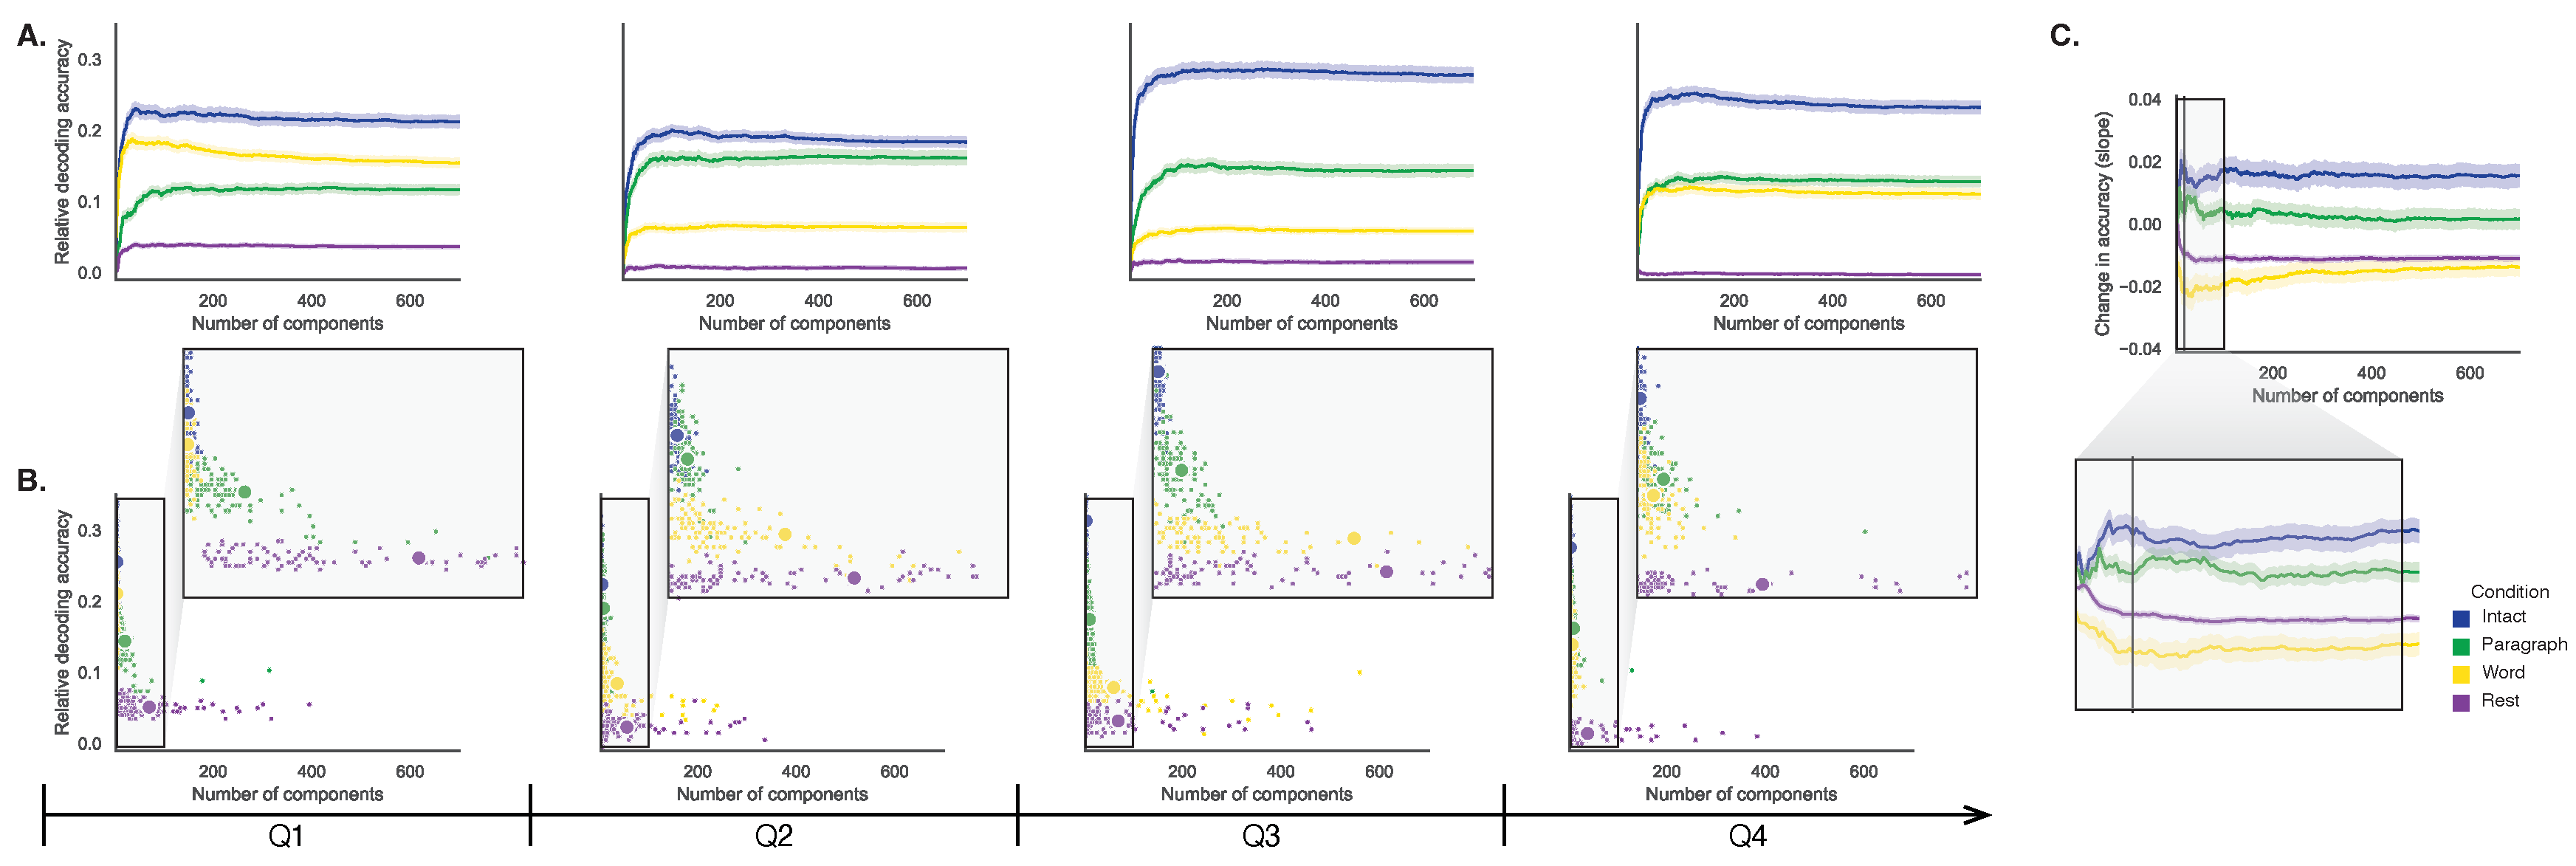
\includegraphics[width=0.8\textwidth]{figs/information_and_compression_over_time}

\caption{\textbf{Changes in decoding accuracy and compression over time.}
\textbf{A. Decoding accuracy by number of components, by story segment.} Each
family of curves is plotted in the same format as Figure~\ref{fig:inflection}A
but reflects data only from one third of the dataset. \textbf{B. Inflection
points by condition and segment.} The dots re-plot the inflection points from
Figure~\ref{fig:inflection}D for reference. The numbers denote the inflection
points for each third of the dataset (1: first third; 2: second third; 3: third
third; colors denote experimental conditions). \textbf{C. Change in decoding
accuracy over time, by number of components.} For each number of components
($x$-axis) and condition (color), we fit a regression line to the decoding
accuracies obtained for the first, second, and third thirds of the dataset
(corresponding to the left, middle, and right columns of Panel A,
respectively). The $y$-axis denotes the slopes of the regression lines. All
error ribbons denote bootstrap-estimated 95\% confidence intervals.}

\label{fig:inflection-thirds}

\end{figure}


If informativeness (to the temporal decoders) and compressibility vary with the
cognitive richness of the stimulus, might these measures also vary over time
\textit{within} a given condition? For example, participants in the intact
condition might process the ongoing story more deeply later on in the story
(compared with earlier in the story) given the additional narrative background
and context they had been exposed to by that point. To examine this
possibility, we divided each condition into three successive time segments. We
computed decoding curves (Fig.~\ref{fig:inflection-thirds}A) and inflection
points (Fig.~\ref{fig:inflection-thirds}B) for each segment and condition. We
found that, in the two most cognitively rich conditions (intact and paragraph),
both decoding accuracy and compressibility, as reflected by the change in
decoding curves, increased with listening time (intact: $t(XXX) = XXX, p =
XXX$; paragraph: $t(XXX) = XXX, p = XXX$). These changes may reflect an
increase in comprehension or depth of processing with listening time. In
contrast, the decoding accuracy and compressibility \textit{decreased} with
listening time in the word condition ($t(XXX) = XXX, p = XXX$) and rest
condition ($t(XXX) = XXX, p = XXX$). This might reflect the depletion of
attentional resources in the less-engaging word and rest conditions.


\begin{figure}[tp]
  \centering
  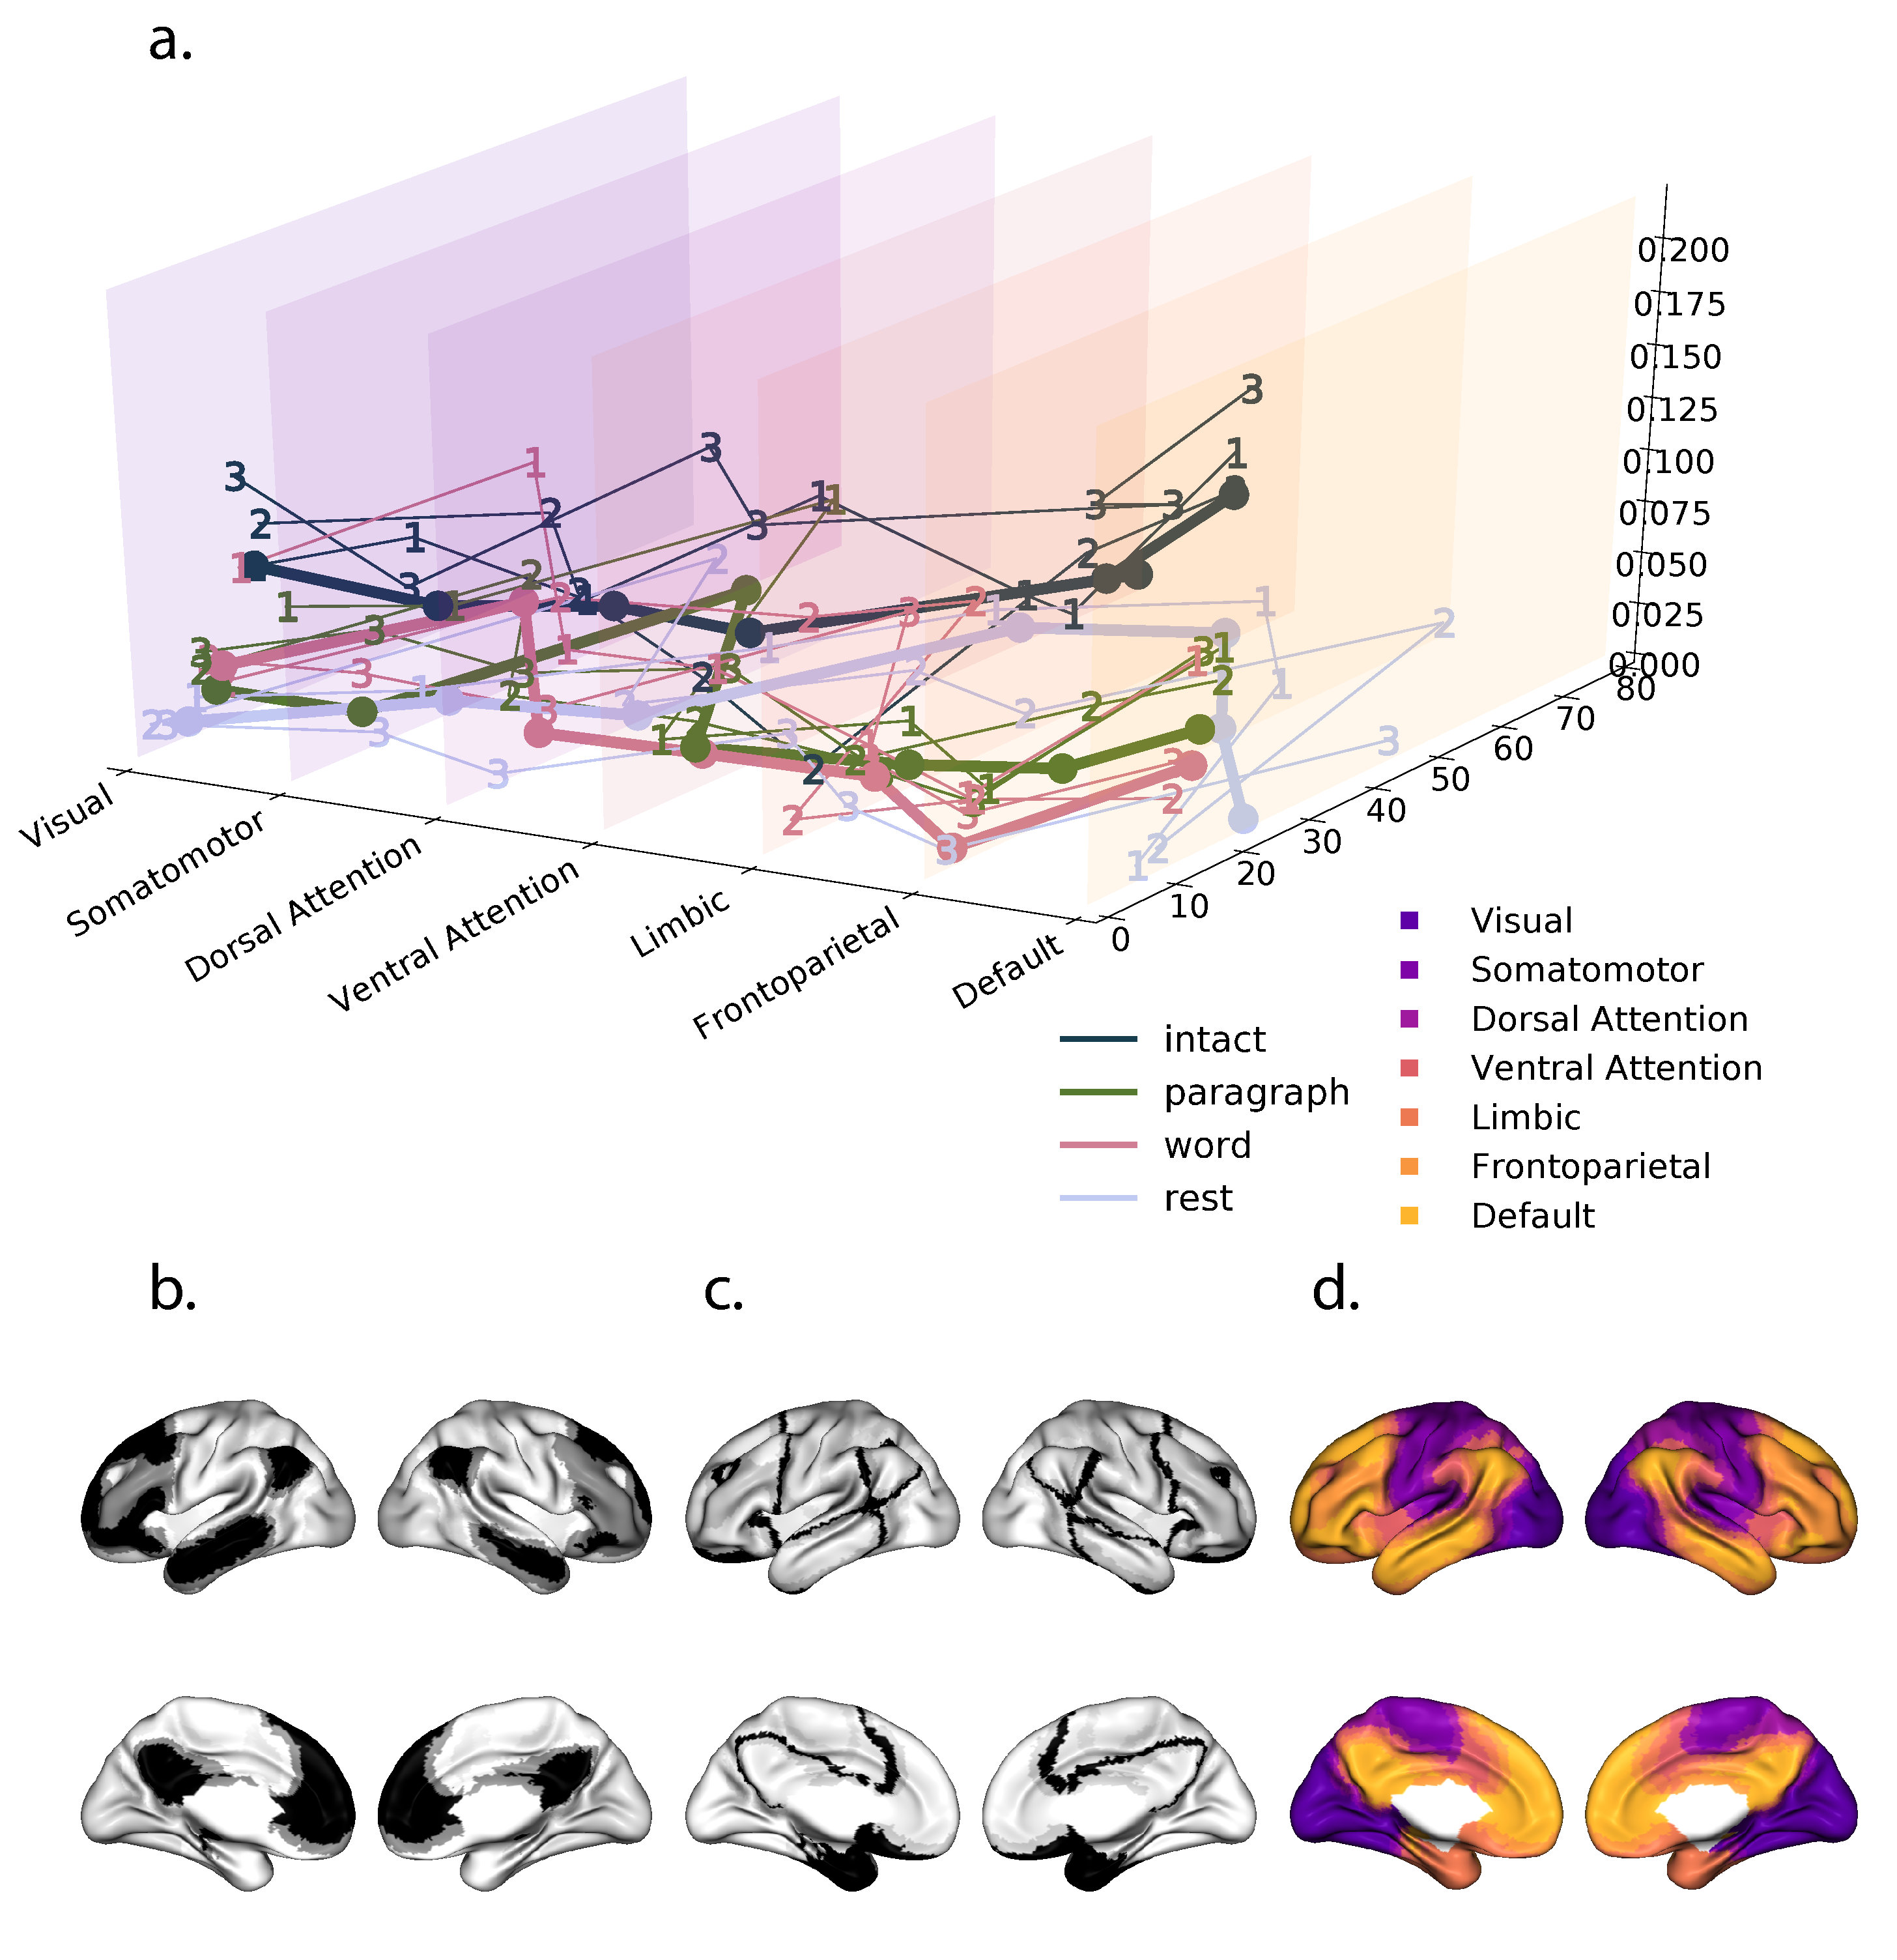
\includegraphics[width=0.7\textwidth]{figs/decode_pcs_network}

  \caption{\textbf{Network-specific decoding accuracy and compression.}
  \textbf{A. Decoding accuracy and number of components for network-specific
  inflection points.} We considered the seven networks identified by
  \cite{YeoEtal11}. We computed each network's inflection point, for each
  experimental condition, using the procedure described in
  Figure~\ref{fig:inflection}C. \textbf{B. Network-specific decoding
  accuracy.} Each of the seven networks are colored according to the decoding
  accuracy at the network's inflection point for the ``intact'' experimental
  condition (corresponding to the dark blue curve in Panel A). \textbf{C.
  Network-specific compression.} Each of the seven networks are colored
  according to the number of components at the network's inflection point for
  the intact experimental condition. Larger numbers of components reflect lower
  compressibility.}

  \label{fig:networks}
\end{figure}

We also wondered how informativeness and compressibility in the different
experimental conditions might vary across brain networks. We used a network
parcellation identified by \cite{YeoEtal11} to segment the brain into seven
distinct networks. The networks can be sorted (roughly) in order from
lower-level to higher-level cortex as follows (Fig.~\ref{fig:networks}A):
visual, somatomotor, dorsal attention, ventral attention, limbic,
frontoparietal, and default mode. Next, we computed decoding curves separately
for the activity patterns within each network and identified each network's
inflection point, for each experimental condition. Moving from low-order
networks to higher-order networks, we found that decoding accuracy (for the
intact condition) tended to increase (Fig.~\ref{fig:networks}B). This suggests
that higher-order networks may carry more content-relevant or stimulus-driven
``information.'' We found no clear trends in the numbers of components at each
network's inflection point across networks or conditions
(Fig.~\ref{fig:networks}C).

\begin{figure}[tp]
  \centering
  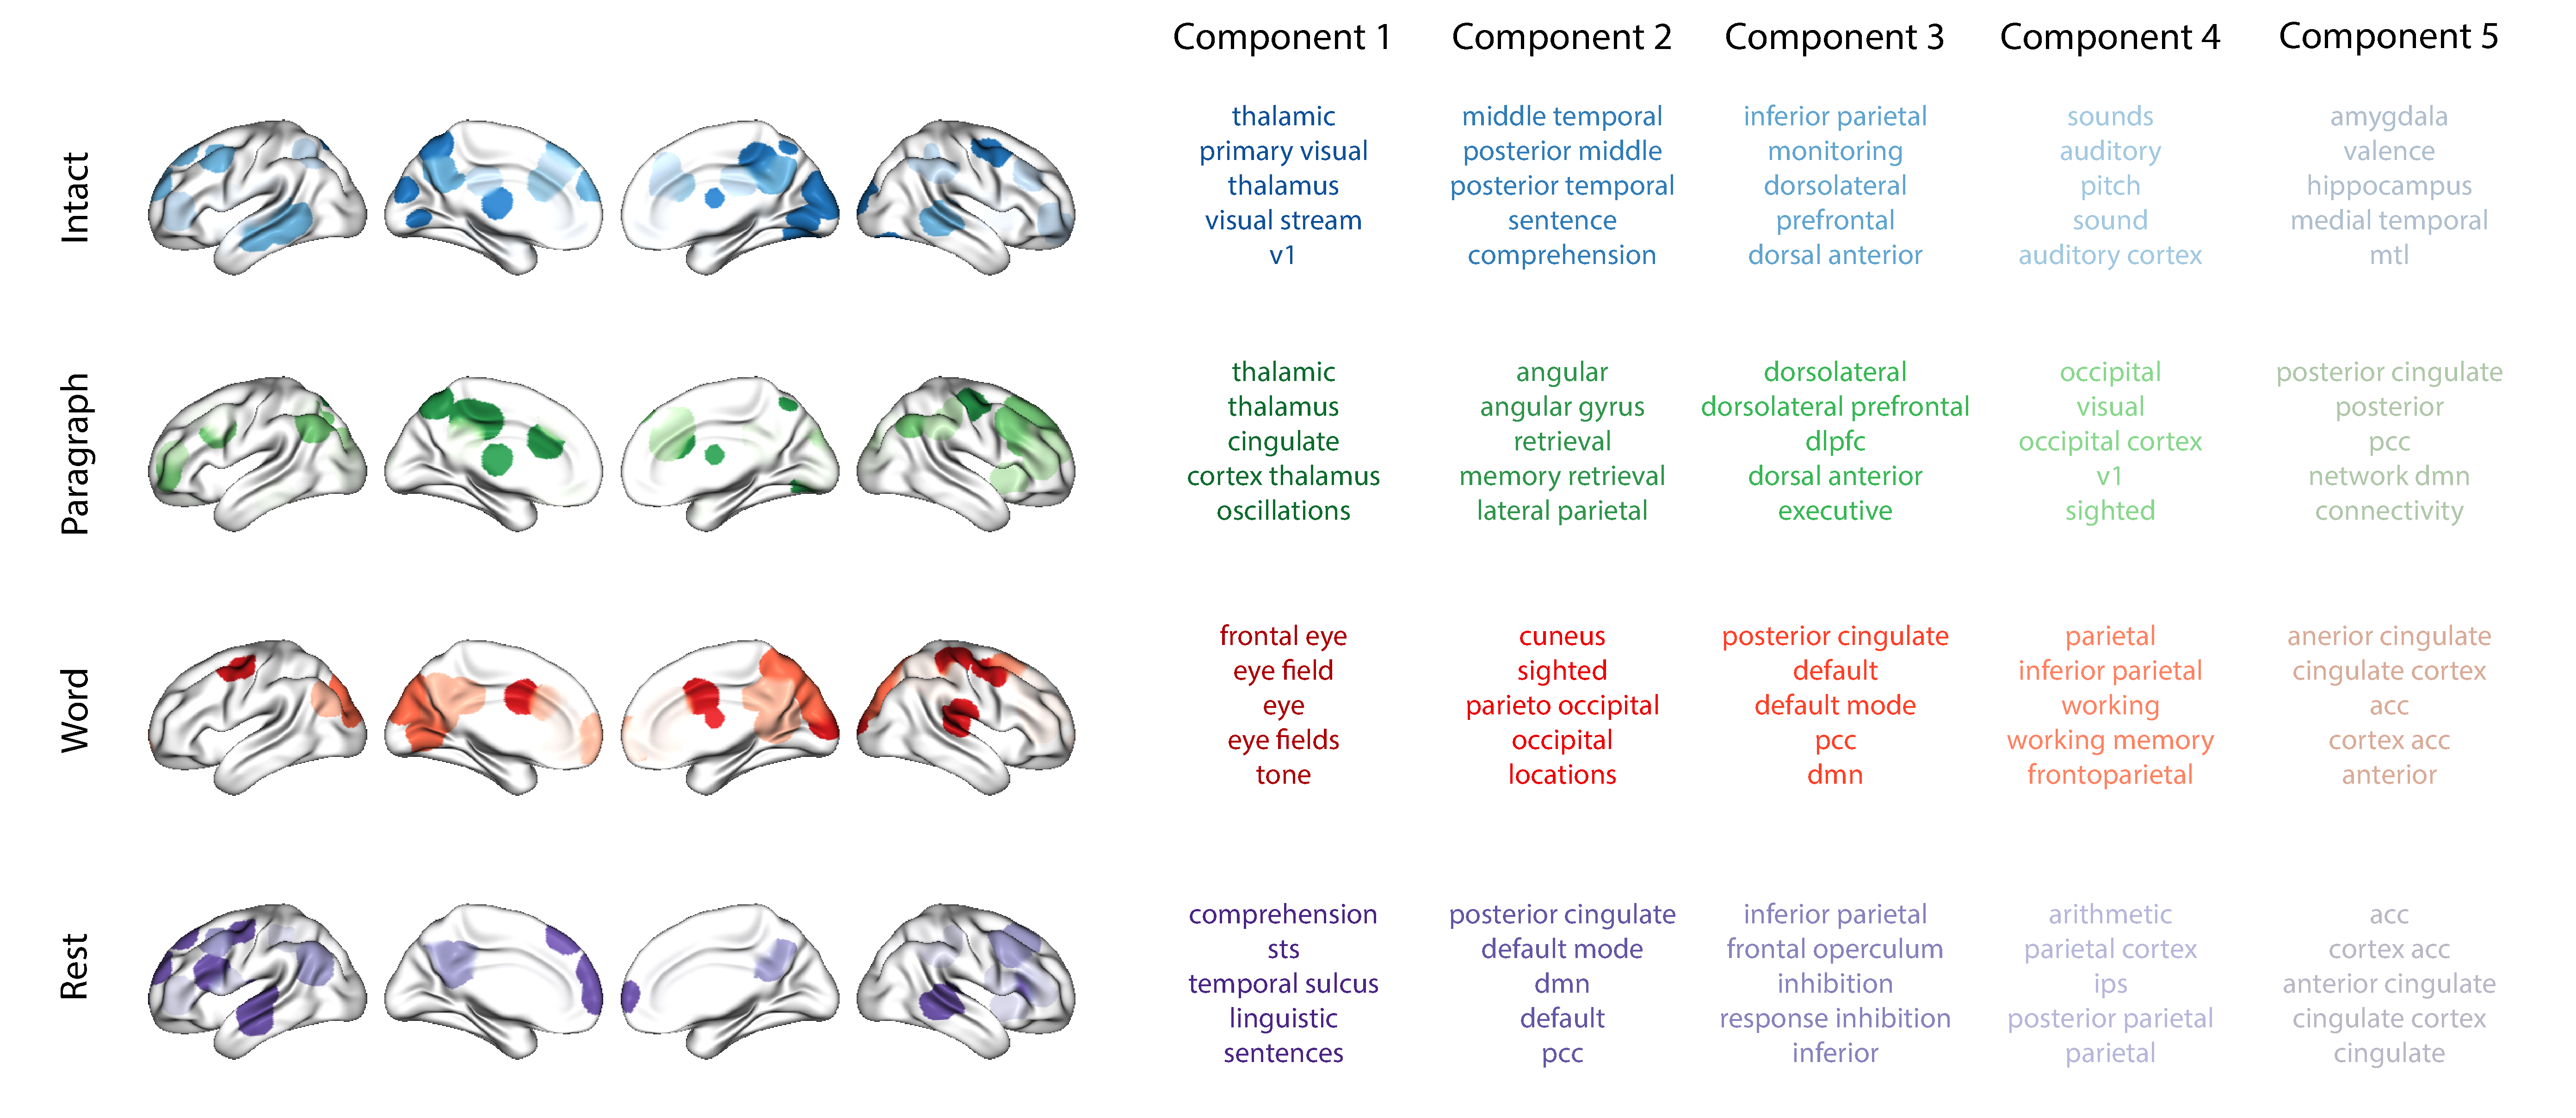
\includegraphics[width=\textwidth]{figs/pca_neurosynth}

\caption{\textbf{Top terms associated with the highest-weighted components by
condition.} Each row corresponds to an experimental condition, and the colors
correspond to the component number (ranked by proportion of variance
explained). The inflated brain plots display the top 20 highest-weighted hubs
(see \textit{Topographic Factor Analysis}) for each components'. The lists on
the right display the top five Neurosynth terms~\citep{RubiEtal17} decoded from
each components' brain map. Analogous maps computed separately for each story
segment may be found in Figure~\synthThirds.}

\label{fig:neurosynth-pca}

\end{figure}

In addition to examining different networks in isolation, we wondered about the
general structure of the full-brain (i.e., potentially multi-network) activity
patterns reflected by different principal components across different
experimental conditions. Figure~\ref{fig:neurosynth-pca} displays inflated
brain maps of the top five highest-weighted components, for each experimental
condition. We also used Neurosynth~\citep{RubiEtal17} to identify, for each
component, the top five terms associated with each map (see \textit{Reverse
inference}). We noticed (by inspection) several common themes across the sets
of terms associated with each component and condition. Memory-related
components included terms like ``middle temporal,'' ``memory retrieval,'' and
``working memory.'' Sensory processing related components included terms like
``primary visual,'' ``auditory cortex,'' ``v1,'' and so on. Other components
were associated with sensory integration (e.g., ``thalamic,'' ``cingulate,''
etc.), sentence comprehension (e.g., ``sentence,'' ``comprehension''), emotion
and valence (e.g., ``amygdala,'' ``valance''), or the default mode network
(e.g., ``default mode'').  The components we identified were relatively stable
across story segments (Fig.~\synthThirds).


\section*{Discussion}

We examined fMRI data collected as participants listened to an auditory
recording of a story, scrambled recordings of the story, or underwent a resting
state scan. We found that cognitively richer stimuli evoked more reliable
(i.e., consistent across people) and information rich brain activity patterns.
The brain patterns evoked by cognitively richer stimuli were also more
compressible, in that each individual component provided more ``signal'' to
temporal decoders relative to components of data from less cognitively rich
conditions (Fig.~\ref{fig:inflection}). Over time (e.g., as the experiment
progressed), these phenomena were strengthened. Specifically, across story
segments, data from more cognitively rich conditions became more informative
and compressible, and data from less cognitively rich conditions became
\textit{less} informative and compressible (Fig.~\ref{fig:inflection-thirds}).
We also repeated these analyses separately for different brain networks. We
found that networks traditionally associated with higher-level cognitive
functions tended to provide more informative brain patterns than networks
traditionally associated with lower level cognitive functions
(Fig.~\ref{fig:networks}). Finally, we examined the most dominant components of
the brain activity patterns from each experimental condition. We used a reverse
inference approach~\citep{RubiEtal17} to identify the terms in the neuroimaging
literature most commonly associated with the corresponding maps. As summarized
in Figure~\ref{fig:discussion}, we found that terms associated with memory and
sensory processing were associated with the strongest components in all three
story listening conditions. Terms associated with sensory integration were
associated with the strongest components in the intact and paragraph-scrambled
conditions. Terms associated with sentence comprehension, emotion, and valence
were associated with the strongest components in the intact condition. Finally,
terms associated with the default mode network were associated with the
strongest components in the word-scrambled and resting state conditions. Taken
together, our findings indicate that the informativeness and compressibility of
our brain activity patterns are task-dependent, and these properties change
systematically with factors like cognitive richness and depth of processing.

\begin{figure}[tp]
  \centering
  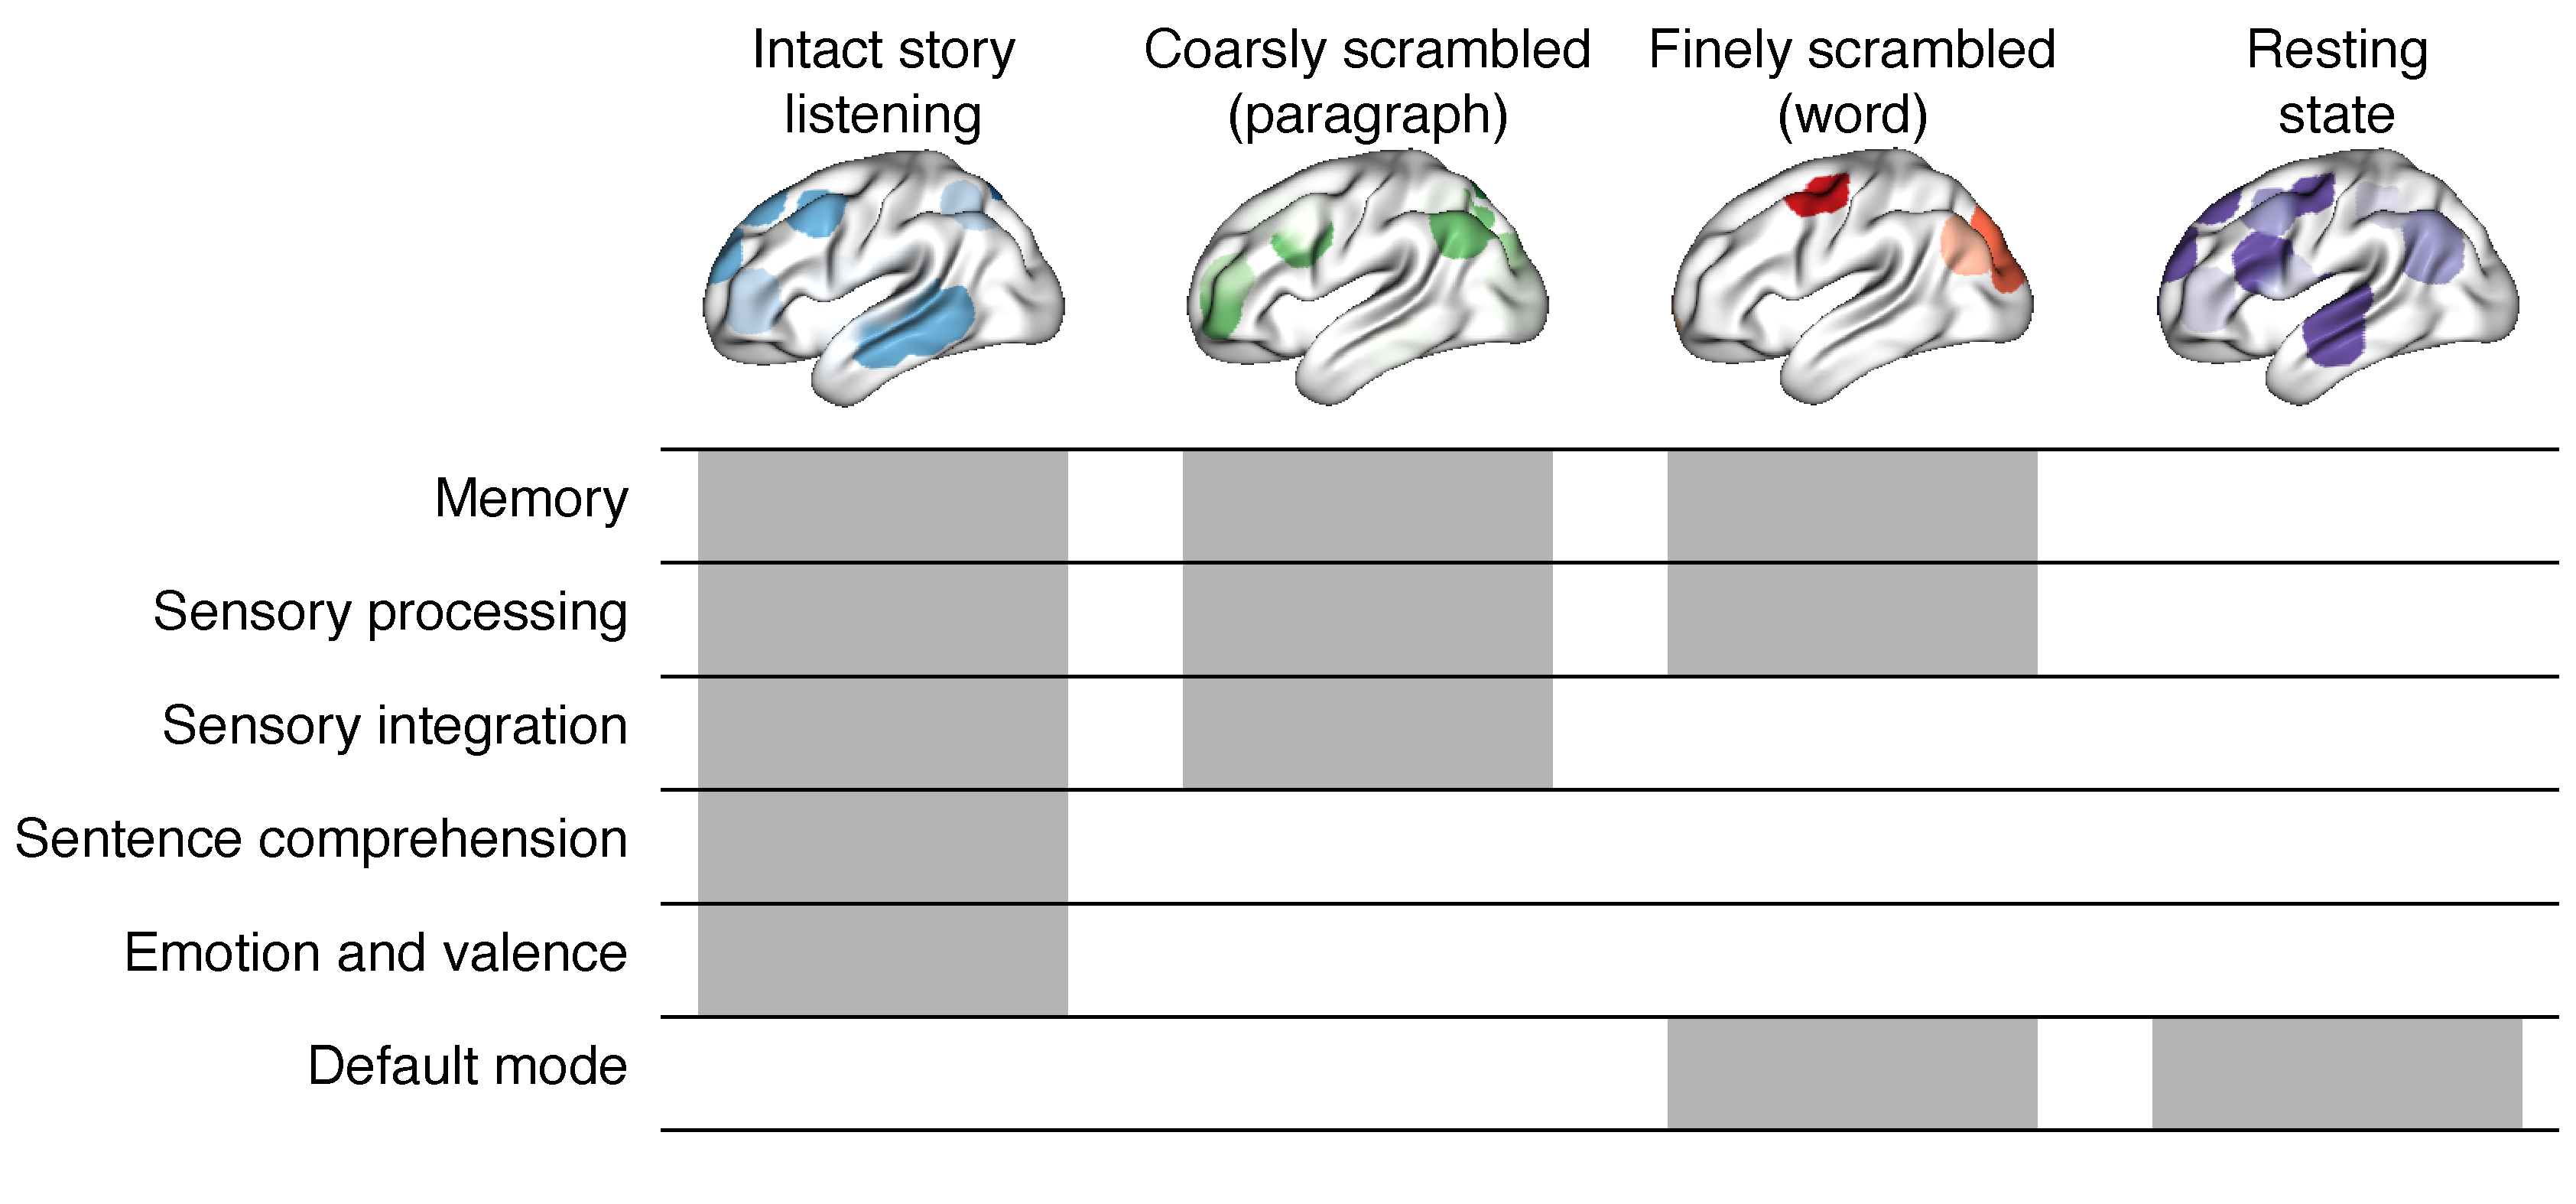
\includegraphics[width=\textwidth]{figs/discussion}

\caption{\textbf{Summary of functions associated with top-weighted components
by condition.} Each column corresponds to an experimental condition. Brain maps
in the top row are reproduced from Figure~\ref{fig:neurosynth-pca}, for
reference. Cognitive functions summarized from the top Neurosynth-derived terms
in Figure~\ref{fig:neurosynth-pca} are listed in the rows on the left.  Shaded cells
denote which experimental conditions were associated with one or more top-weighted
principal components associated with the given function.}

\label{fig:discussion}
\end{figure}

Our explorations of informativeness and compressibility are related to a much
broader literature on the correlational and causal structure of brain activity
patterns~\citep{PretEtal17, OwenEtal21, RogeEtal07, RubiSpor10, SizeEtal18,
SmitEtal13b, SmitEtal13c, SrinEtal07, TomaVolk11, YeoEtal11, AdacEtal12,
BassSpor17, BullSpor09, SporHone06, SporBetz16, SporZwi04, DhamEtal08,
KorzEtal08, BrovEtal04}. Correlations or causal associations between different
brain regions simultaneously imply that full-brain activity patterns will be
compressible and also that those activity patterns will contain redundancies.
For example, the extent ot which activity patterns at one brain area can be
inferred or predicted from activity patterns at other
areas~\citep[e.g.,][]{OwenEtal20, ScanEtal21}, reflects overlap in the
information available in or represented by those brain areas. If brain patterns
in one area are recoverable using brain patterns in another area, then the
``signal'' used to convey the activity patterns could be compressed by removing
the recoverable activity. Predictable (and therefore redundant) brain activity
patterns are also more robust to signal corruption. For example, even if the
activity patterns at one region are unreadable or unreliable at a given moment,
that unreliability could be compensated for by other regions' activity patterns
that were predictive of the unreliable region.

Our findings that informativeness and compressibility change with task demands
may follow from task-dependent changes in full-brain correlation patterns. A
number of prior studies have found that so-called ``functional connectivity''
(i.e., correlational) patterns vary reliably across tasks, events, and
situations~\citep{SimoEtal16, ColeEtal14, SmitEtal09, OwenEtal21}. By examining
how these task-dependent changes in correlations affect informativeness and
compressibility, our work suggests a potential reason why the statistical
structure of brain activity patterns might vary with cognitive task or with
cognitive demands. For lower-level tasks, or for tasks that require relatively
little ``deep'' cognitive processing, our brains may optimize activity patterns
for robustness and redundancy over expressiveness, for example to maximize
reliability. For higher-level tasks, or for tasks that require deeper cognitive
processing, our brains may sacrifice some redundancy in favor of greater
expressiveness.

In the information theory sense~\citep{Shan48}, when a signal is transmitted
using a fixed alphabet of ``symbols,'' the information rate decreases as the
signal is compressed (e.g., fewer symbols transmitted per unit time, using an
alphabet with fewer symbols, etc.). Our finding that each individual brain
component (symbol) becomes more informative as cognitive richness increases
suggests that the ``alphabet'' of brain activity patterns is also
task-dependent. Other work suggests that the representations that are
\textit{reflected} by brain activity patterns may also change with task
demands. For example, our brains may represent the same perceptual stimulus
differently depending on which aspects of the stimulus or which combinations of
features are task-relevant~\citep{MackEtal20}.

Different brain networks also varied in how informative and compressible their
activity patterns were across experimental conditions (e.g.,
Fig.~\ref{fig:networks}). This might follow from evolutionary optimizations
that reflect the relevant constraints or demands placed on those networks. One
possibility is that cortex is organized in a hierarchy of networks ``concerned
with'' or selective to different levels of processing or function. To the
extent that different levels of processing (e.g., low-level sensory processing
versus ``deeper'' higher-level processing) reflect different stimulus
timescales~\citep[e.g.,][]{Mann20}, the network differences we observed might
also relate to the timescales at which each network is maximally
sensitive~\citep{RegeEtal18, BaldEtal17,LernEtal11, HassEtal08}.

\subsection*{Concluding remarks}

Cognitive neuroscientists are still grappling with basic questions about the
fundamental ``rules'' describing how our brains respond, and about how brain
activity patterns and the associated underlying cognitive representations and
computations are linked. We identified two aspects of brain activity patterns,
informativeness and compressibiilty, that appear to change systematically with
task demands and across brain networks. Our work helps to clarify how the
``neural code'' might be structured, and how the code might vary across tasks
and brain areas.

\section*{Methods}

We measured properties of recorded neuroimaging data under different task
conditions that varied systematically in cognitive engagement and depth of
processing. We were especially interested in how \textit{informative} and
\textit{compressible} the activity patterns were under these different
conditions (Fig.~\ref{fig:information-compression}).


\subsection*{Functional neuroimaging data collected during story
  listening}

We examined an fMRI dataset collected by \cite{SimoEtal16} that the authors
have made publicly available at
\href{http://arks.princeton.edu/ark:/88435/dsp015d86p269k}{arks.princeton.edu/ark:/88435/dsp015d86p269k}.
The dataset comprises neuroimaging data collected as participants listened to
an audio recording of a story (intact condition; 36 participants), listened to
temporally scrambled recordings of the same story (17 participants in the
paragraph-scrambled condition listened to the paragraphs in a randomized order
and 36 in the word-scrambled condition listened to the words in a randomized
order), or lay resting with their eyes open in the scanner (rest condition; 36
participants). Full neuroimaging details may be found in the original paper for
which the data were collected~\citep{SimoEtal16}. Procedures were approved by
the Princeton University Committee on Activities Involving Human Subjects, and
by the Western Institutional Review Board (Puyallup, WA). All subjects were
native English speakers with normal hearing and provided written informed
consent.

\subsection*{Hierarchical topographic factor analysis (HTFA)}

Following our prior related work, we used HTFA~\citep{MannEtal18} to derive a
compact representation of the neuroimaging data. In brief, this approach
approximates the timeseries of voxel activations (44,415 voxels) using a much
smaller number of radial basis function (RBF) nodes~\citep[in this case, 700
nodes, as determined by an optimization procedure;][]{MannEtal18}). This
provides a convenient representation for examining full-brain activity patterns
and network dynamics. All of the analyses we carried out on the neuroimaging
dataset were performed in this lower-dimensional space. In other words, each
participant's data matrix was a number-of-timepoints ($T$) by 700 matrix of
HTFA-derived factor weights (where the row and column labels were matched
across participants). Code for carrying out HTFA on fMRI data may be found as
part of the BrainIAK toolbox~\citep{CapoEtal17, KumaEtal21}, which may be
downloaded at \href{https://brainiak.org/}{brainiak.org}.

\subsection*{Principal components analysis (PCA)}

We applied group PCA~\citep{SmitEtal14} separately to the HTFA-derived
representations of the data (i.e., factor loadings) from each experimental
condition. Specifically, for each condition, we considered the set of all
participants' $T$ by 700 factor weight matrices. We used group PCA to project
these 700-dimensional matrices into a series of shared $k$-dimensional spaces,
for $k \in \{3, 4, 5, ..., 700\}$. This yielded a set of number-of-participants
matrices, each with $T$ rows and $k$ columns.

\subsection*{Temporal decoding}

We sought to identify neural patterns that reflected participants' ongoing
cognitive processing of incoming stimulus information. As reviewed by
\cite{SimoEtal16}, one way of homing in on these stimulus-driven neural
patterns is to compare activity patterns across individuals. In particular,
neural patterns will be similar across individuals to the extent that the
neural patterns under consideration are stimulus-driven, and to the extent that
the corresponding cognitive representations are reflected in similar spatial
patterns across people~\citep{SimoChan20}. Following this logic, we used an
across-participant temporal decoding test developed by \cite{MannEtal18} to
assess the degree to which different neural patterns reflected ongoing
stimulus-driven cognitive processing across people. The approach entails using
a subset of the data to train a classifier to decode stimulus timepoints (i.e.,
moments in the story participants listened to) from neural patterns. We use
decoding (forward inference) accuracy on held-out data, from held-out
participants, as a proxy for the extent to which the inputted neural patterns
reflected stimulus-driven cognitive processing in a similar way across
individuals.

\subsubsection*{Forward inference and decoding accuracy}

We used an across-participant correlation-based classifier to decode which
stimulus timepoint matched each timepoint's neural pattern. For a given value
of $k$ (i.e., number of principal components), we first used group PCA to
project the data from each condition into a shared $k$-dimensional space. Next,
we divided the participants into two groups: a template group,
$\mathcal{G}_{\mathrm{template}}$ (i.e., training data), and a to-be-decoded
group, $\mathcal{G}_{\mathrm{decode}}$ (i.e., test data). We averaged the
projected data within each group to obtain a single $T$ by $k$ matrix for each
group. Next, we correlated the rows of the two averaged matrices to form a $T$
by $T$ decoding matrix, $\mathbf{\Lambda}$. In this way, the rows of
$\mathbf{\Lambda}$ reflected timepoints from the template group, while the
columns reflected timepoints from the to-be-decoded group. We used
$\mathbf{\Lambda}$ to assign temporal labels to each timepoint (row) from the
test group's matrix, using the row of the training group's matrix with which it
was most highly correlated. We repeated this decoding procedure, but using
$\mathcal{G}_{\mathrm{decode}}$ as the template group and
$\mathcal{G}_{\mathrm{template}}$ as the to-be-decoded group. Given the true
timepoint labels (for each group), we defined the decoding accuracy as the
average proportion of correctly decoded timepoints, across both groups (where
chance perfomance is $\frac{1}{T}$). In Figures~\ref{fig:inflection}
and~\ref{fig:inflection-thirds} we report the decoding accuracy for each
condition and value of $k$, averaged across $n = 100$ cross validation folds.

\subsection*{Reverse inference}

To help interpret the brain activity patterns we found within the contexts of
other studies, we created summary maps of each principal component, for each
experimental condition, by summing together the 20 HTFA-derived RBF nodes (see
\textit{Hierarchical Topographic Factor Analysis}) with the highest absolute
value weights for each of the top 5 components (Figs.~\ref{fig:neurosynth-pca},
\synthThirds). We then carried out a meta analysis using
Neurosynth~\citep{RubiEtal17} to identify the 5 terms most commonly associated
with the given map.


\section*{Data and code availability}

All of the code used to produce the figures and results in this manuscript,
along with links to the corresponding data, may be found at
\href{https://github.com/ContextLab/pca_paper}{github.com/ContextLab/pca\_paper}.

\section*{Acknowledgements} 

We acknowledge discussions with Rick Betzel, Luke Chang, Emily Finn, and Jim
Haxby. Our work was supported in part by NSF CAREER Award Number 2145172 to
J.R.M. The content is solely the responsibility of the authors and does not
necessarily represent the official views of our supporting organizations. The
funders had no role in study design, data collection and analysis, decision to
publish, or preparation of the manuscript.


\section*{Author contributions} 

Conceptulization: J.R.M. and L.L.W.O. Methodology: J.R.M. and L.L.W.O.
Implementation: L.L.W.O. Analysis: L.L.W.O. Writing, Reviewing, and Editing:
J.R.M. and L.L.W.O. Supervision: J.R.M.

\bibliographystyle{apacite}
\bibliography{CDL-bibliography/cdl}

\end{document}


